\documentclass[11pt,]{article}
\usepackage{lmodern}
\usepackage{amssymb,amsmath}
\usepackage{ifxetex,ifluatex}
\usepackage{fixltx2e} % provides \textsubscript
\ifnum 0\ifxetex 1\fi\ifluatex 1\fi=0 % if pdftex
  \usepackage[T1]{fontenc}
  \usepackage[utf8]{inputenc}
\else % if luatex or xelatex
  \ifxetex
    \usepackage{mathspec}
  \else
    \usepackage{fontspec}
  \fi
  \defaultfontfeatures{Ligatures=TeX,Scale=MatchLowercase}
\fi
% use upquote if available, for straight quotes in verbatim environments
\IfFileExists{upquote.sty}{\usepackage{upquote}}{}
% use microtype if available
\IfFileExists{microtype.sty}{%
\usepackage{microtype}
\UseMicrotypeSet[protrusion]{basicmath} % disable protrusion for tt fonts
}{}
\usepackage[margin=1.0in]{geometry}
\usepackage{hyperref}
\hypersetup{unicode=true,
            pdftitle={The microbiota of the proximal and distal human colon},
            pdfborder={0 0 0},
            breaklinks=true}
\urlstyle{same}  % don't use monospace font for urls
\usepackage{graphicx,grffile}
\makeatletter
\def\maxwidth{\ifdim\Gin@nat@width>\linewidth\linewidth\else\Gin@nat@width\fi}
\def\maxheight{\ifdim\Gin@nat@height>\textheight\textheight\else\Gin@nat@height\fi}
\makeatother
% Scale images if necessary, so that they will not overflow the page
% margins by default, and it is still possible to overwrite the defaults
% using explicit options in \includegraphics[width, height, ...]{}
\setkeys{Gin}{width=\maxwidth,height=\maxheight,keepaspectratio}
\IfFileExists{parskip.sty}{%
\usepackage{parskip}
}{% else
\setlength{\parindent}{0pt}
\setlength{\parskip}{6pt plus 2pt minus 1pt}
}
\setlength{\emergencystretch}{3em}  % prevent overfull lines
\providecommand{\tightlist}{%
  \setlength{\itemsep}{0pt}\setlength{\parskip}{0pt}}
\setcounter{secnumdepth}{0}
% Redefines (sub)paragraphs to behave more like sections
\ifx\paragraph\undefined\else
\let\oldparagraph\paragraph
\renewcommand{\paragraph}[1]{\oldparagraph{#1}\mbox{}}
\fi
\ifx\subparagraph\undefined\else
\let\oldsubparagraph\subparagraph
\renewcommand{\subparagraph}[1]{\oldsubparagraph{#1}\mbox{}}
\fi

%%% Use protect on footnotes to avoid problems with footnotes in titles
\let\rmarkdownfootnote\footnote%
\def\footnote{\protect\rmarkdownfootnote}

%%% Change title format to be more compact
\usepackage{titling}

% Create subtitle command for use in maketitle
\newcommand{\subtitle}[1]{
  \posttitle{
    \begin{center}\large#1\end{center}
    }
}

\setlength{\droptitle}{-2em}
  \title{The microbiota of the proximal and distal human colon}
  \pretitle{\vspace{\droptitle}\centering\huge}
  \posttitle{\par}
  \author{}
  \preauthor{}\postauthor{}
  \date{}
  \predate{}\postdate{}

\usepackage{setspace}
\doublespacing
\usepackage{lineno}
\linenumbers
\renewcommand{\familydefault}{\sfdefault}
\usepackage{graphicx}

\begin{document}
\maketitle

\vspace{35mm}

Running title: The microbiome of the proximal and distal human colon

\vspace{35mm}

Kaitlin J. Flynn\textsuperscript{1}, Charles C.
Koumpouras\textsuperscript{1}, Mack T. Ruffin IV\textsuperscript{2},
Danielle Kimberly Turgeon\textsuperscript{3\(\dagger\)}, and Patrick D.
Schloss\textsuperscript{1\(\dagger\)}

\vspace{35mm}

\(\dagger\) Corresponding authors:
\href{mailto:kturgeon@med.umich.edu}{\nolinkurl{kturgeon@med.umich.edu}}
and \href{mailto:pschloss@umich.edu}{\nolinkurl{pschloss@umich.edu}}

1. Department of Microbiology and Immunology, University of Michigan
Medical School, Ann Arbor, Michigan 48109

2. Pennslyvania State University, Hershey, Pennslyvania ??

3. Department of Internal Medicine, Division of Gastroenterology,
University of Michigan Medical School, Ann Arbor, Michigan

\newpage

\subsubsection{Abstract}\label{abstract}

Chemical and nutrient gradients along the human colon create
microenvironments that affect the distrubution and composition of the
gut microbiota. The microbiome has been implicated in colorectal cancer
(CRC) and inflammatory bowel disease (IBD). Further, these diseases
exhibit different symptoms depending on the location of the colon they
are found in. CRC tumors of the proximal and distal colon are
morphologically and genetically distinct. Similarly, inflammatory bowel
diseases such as Crohn's are typically exacerbated in the proximal
instestine while ulcerative colitis patients often experience symptoms
in the distal colon. Previous analysis of the fecal microbiota from
healthy and CRC or IBD patients has revealed different microbial
signatures associated with these diseases. We extended these
observations of the fecal microbiome to include analysis of the proximal
and distal healthy human colon. We used a two-colonoscope approach on
subjects that had not undergone standard bowel preparation procedure. In
contrast to previous efforts using prepared colonoscopy, this technique
allowed us to characterize the native proximal and distal luminal and
mucosal microbiome without prior chemical disruption. 16S rRNA gene
sequencing was performed on proximal and distal mucosal and luminal
biopsies and home-collected stool for 20 healthy individuals. Diversity
analysis revealed that each site contained a diverse community and that
a patient's samples were more similar to each other than to that of
other individuals. A patient's feces were most similar to samples taken
from the distal lumen, likely reflecting the anatomical structure of the
colon. Since we could not differentiate the communities in the proximal
and distal colon based on community structure or community membership
alone, we employed the Random Forest machine-learning algorithm to
identify key taxa that the two sites in the lumen and mucosa. Random
Forest classification models were built using taxa abundance and sample
location and revealed distinct populations that were found in each
location. A model differentiating the proximal mucosa and lumen was
built with an AUC of 0.856. The proximal mucosa had a higher abundance
of the genera \emph{Enterobacteriaceae} and \emph{Bacteriodes}.
\emph{Peptoniphilus, Anaerococcus, Finegoldia,} and \emph{Turicibacter}
were most likely to be found in distal mucosal samples versus distal
luminal samples (AUC = 0.975). The classification model performed well
(AUC = 0.920) when classifying mucosal samples into proximal or distal
sides, but separating luminal samples from each side proved more
challenging (AUC = 0.575). The distal mucosa was found to have high
populations of \emph{Finegoldia, Murdochiella} and \emph{Porphyromonas}.
Proximal and distal luminal samples were comprised of many of the same
taxa, likely reflecting the fact that stool moves along the colon from
the proximal to distal end. By sampling the unprepped human colon, our
results have identified distinct bacterial populations native to the
proximal and distal sides. Further investigation of these bacteria may
elucidate if and how these groups contribute to different pathogenesis
processes on the respective sides of the colon.

\paragraph{wordcount?}\label{wordcount}

\subsubsection{Introduction}\label{introduction}

The human colon is an ecosystem comprised of several different
microenvironments inhabited by resident bacterial members of the
microbiome. Concentrations of oxygen, water and anti-microbial peptides
change along the gut axis and influence what populations of microbes
reside in each location. Microenvironments differ not only
longitutinally along the colon, but latitudinally from the epithelium to
mucosa to intestinal lumen, offering several sites for different
microbial communities to flourish. The identity of these specific
microbes and communities are important for understanding the etiology of
complex colon diseases such as Inflammatory Bowel Disease (IBD) and
Colorectal Cancer (CRC). IBD and CRC are known to be preceded or
accelerated by perturbations in gut microbes (1--3). The severity,
symptoms, morbidity and mortality of these diseases is known to vary
based upon the biogeographical location in which they occur. For
instance, CRC tumors that arise on the distal side of the colon are
infiltrating lesions that present with painful symptoms (4). In
contrast, 47\% of CRCs are caused by proximal-sided colon tumors that
are sessile and form along the wall of the colon, often remaining
asymptomatic until advanced carcinogenesis (4). The distal and proximal
sides of the colon differ in the amount of inflammation present and the
genomic instability of precancerous cells, respectively, in addition to
variation in the previously mentioned chemical gradients (1, 5, 6). In
IBD patients, disease flares in the distal colon are usually indicative
of ulcerative colitis (UC), whereas Crohn's disease (CD) patients
typically experience disease in the small intestine, ileum and proximal
colon (2). UC presents as large and highly inflammed mucosal ulcers,
where as CD lesions are often smaller and have areas of normal tissue
distributed amongst the flare (2). Thus, given the varied physiology of
the proximal-distal axis of the colon and known differences in disease
patterns at these sites, symbiotic microbes and their metabolites likely
vary as well, and may influence the heterogenous disease prognoses of
IBD and CRC. Because CRC can be a long-term complication of IBD, the
distribution of microbes is important to understanding the
pathophysiology of both diseases.

Several recent findings have shown that development and progression of
IBD or CRC can be attributed to specific molecular events as a result of
interactions between the gut microbiota and human host (1, 3). For
instance, comparison of the bacteria present on CRC tumors with those
found on nearby healthy tissue has identified specific species that are
tumor-associated (7). These species include the oral pathogens
\emph{Fusobacterium nucleatum} and \emph{Porphyromonas asacharolytica}.
Interestingly, these periodontal pathogens have been highly predictive
of whether a patient had CRC tumors or not in our prior human stool
classification studies (8). \emph{F. nucleatum} has also been found to
be elevated in the stool and biopsies of patients with IBD as compared
to healthy controls (9). Furthermore, studies of \emph{F. nucleatum}
isolated from mucosal biopsies showed that more invasive \emph{F.
nucleatum} positively correlates with IBD disease level (9). Like many
intestinal pathogens, the bacteria appear to have a high-impact despite
being lowly-abundant in the community (2). The physiology of these rare
taxa may contribute to the colonic disease state. These studies often
examined only shed human stool or the small intestine, preventing
fine-resolution analysis of paired samples from the proximal and distal
sides of the colon. Similarly, comparisons of on- or off-tumor/lesion
bacteria rarely have matched tissue from the other side of the colon
from the same patient, limiting what conclusions can be drawn about the
colonic microbiome overall, let alone at that specific site. Due to
these limitations, the contribution of the gut microbiota to IBD and CRC
disease location in the colon is largely undefined. Characterizing these
communities could provide needed insight into disease etiology,
including how the disruption of the healthy community could promote the
initiation or proliferation of the distinct proximal and distal CRC
tumors or IBD flares.

The few existing profiles of the microbial biogeography of the gut have
been limited by sample collection methods. The majority of human gut
microbiome studies have been performed on whole shed feces or on samples
collected during colonoscopy procedures. While the latter method allows
investigators to acquire samples from inside the human colon, typically
this procedure is preceded by the use of bowel preparation methods such
as the consumption of laxatives to cleanse the bowel. Bowel preparation
is essential for detecting cancerous or precancerous lesions in the
colon, but complicates microbiome profiling as the chemicals strip the
bowel of contents and disrupt the mucosal layer (10, 11). As such, what
little information we do have about the biogeographical distribution of
the microbes in the proximal and distal colon is confounded by the bowel
preparation procedure.

Here we address the limitations of previous studies and effectively
identify the microbes specific to the lumen and mucosa of the proximal
and distal healthy human colon. We used an unprepared colonoscopy
technique to sample the natural community of each location of the gut
without prior disruption of the native bacteria in 20 healthy
volunteers. To address the inherent inter-individual variation in human
microbiomes, we used a machine-learning classification algorithm trained
on curated 16S rRNA sequencing reads to identify microbes specific to
each location. We found that our classification models were able to
separate mucosal and lumenal samples as well as differentiate between
sides of the colon based on populations of specific microbes. By
identifying the specific microbes we are poised to ask if and how the
presence or disruption of the microbes at each site contribute to the
development of the specific tumor subtypes of CRC in the proximal and
distal human colon.

\subsubsection{Results}\label{results}

\paragraph{Microbial membership and diversity of the proximal and distal
colon}\label{microbial-membership-and-diversity-of-the-proximal-and-distal-colon}

Lumenal and mucosal samples were collected from the proximal and distal
colon of 20 healthy humans that had not undergone bowel preparation
(Figure 1). Participants also collected stool at home one week prior to
the procedure. To characterize the bacterial communities present at
these sites, 16S rRNA gene sequencing was performed on extracted DNA
from each sample. As expected, each site was primarily dominated by
\emph{Firmicutes} and \emph{Bacteriodetes} (Figure 2A) (12). Samples had
varying levels of diversity at each site, irrespective of the individual
(Figure 2B). For example, the proximal mucosa was more diverse than the
distal for some individuals while the opposite was true for others.
Therefore we could not identify a clear pattern of changes in microbial
diversity along the gut axis.

To compare similarity between sides (proximal or distal) or sites (lumen
or mucosa), we calculated distances from Operational Taxonomic Unit
(OTU) abundances and compared these distances for all individuals.
Again, across all patient samples we observed a range of distances when
comparing sample locations (Figure 3A) and again those ranges did not
follow a clear pattern on an individual basis. However, when comparing
median distances between the proximal lumen and mucosa, the proximal
versus distal lumen, the proximal versus distal mucosa, and the distal
lumen and mucosa, we found that the proximal lumen and mucosa were most
similar to each other than the other samples (P \textless{} 0.005,
Wilcoxon, BH adjustment).

\paragraph{Fecal samples resemble lumenal samples from the distal
colon}\label{fecal-samples-resemble-lumenal-samples-from-the-distal-colon}

Next, we calculated distances to examine how each sample compared to the
home-collected feces. Amidst variability between patients, we did
identify significantly smaller distance between the distal lumenal
sample and the feces (Figure 3B, P \textless{} 0.05, Wilcoxon, BH
adjustment). Furthermore, there was an even larger difference in the
comparisons of the distal mucosa to the feces, indicating that the
mucosa is different from the stool as compared to lumen (P \textless{}
0.0005, Wilcoxon, BH adjustment). To determine what factors may be
driving the differences seen among the samples, we compared distances
between samples from all subjects (interpersonal) versus samples from
within one subject (intrapersonal). We found that samples from one
individual were far more similar to each other than to other study
subjects (Figure 3C), consistent with previous human microbiome studies
that have sampled multiple sites of the human colon (13--15). Thus
interpersonal variation between subjects drove the differences between
samples more than sample site or location. Overall, the results
comparing the structure of the communities suggest that the contents of
the distal lumen are most representative of the patient's feces, and the
microbes remaining on the mucosa are more distinct.

\paragraph{Random Forest classification models identify important
Operational Taxonomic Units (OTUs) on each
side}\label{random-forest-classification-models-identify-important-operational-taxonomic-units-otus-on-each-side}

To identify OTUs that were distinct at each biogeographical site, we
constructed several Random Forest models trained using OTU abundances.
We used 10-fold cross validation to build the first model to classify
the lumenal versus mucosal samples for the proximal and distal sides,
independently (Figure S1A). The models were constructed to only use the
five most predictive OTUs as input to reduce overfitting between
samples. The models performed well when classifying these samples (AUC =
0.856 and AUC = 0.975, respectively). The OTUs that were most predictive
of each site were identified by their greatest mean decrease in accuracy
when removed from the model. For distinguishing the proximal lumen and
mucosa, OTUs from the \emph{Bacteriodes}, \emph{Actinomyces},
\emph{Psuedomonas} and two OTUs from the \emph{Enterobacteraceae} genera
were differentially abundant (Figure 4A). The model classifying the
distal lumen and mucosa identified OTUs from \emph{Turicibacter},
\emph{Finegoldia}, \emph{Peptoniphilus} and two OTUs from the
\emph{Anaerococcus} genera (Figure 4B). These results indicated that
there were fine differences between the different sites of the colon,
and that these could be traced to specific OTUs on each side.

Next, we built a model to differentiate the proximal and distal lumenal
samples using 10-fold cross validation. The model performed best when
distinguishing the proximal versus distal mucosa (Figure S1B, AUC =
0.920) compared to the proximal versus distal lumen (AUC = 0.575). These
models were also constructed to use only the five most predictive OTUs
as input to reduce overfitting. OTUs that were differentially abundant
between the distal and proximal mucosa included members of the
\emph{Porphyromonas}, \emph{Murdochiella}, \emph{Finegoldia},
\emph{Anaerococcus} and \emph{Peptoniphilus} genera (Figure 5A).
Differentially abundant OTUs of the proximal and distal lumen included
three OTUs of the \emph{Bacteroides} genus, a \emph{Clostridium IV} OTU
and an \emph{Oscillibacter} OTU (Figure 5B). This analysis found that
some of the same OTUs that are distinct between the mucosa and lumen
also helped to differentiate between the two sides- such as
\emph{Anaerococcus} and \emph{Finegoldia}.

\paragraph{Bacterial OTUs associated with cancer are found in healthy
individuals}\label{bacterial-otus-associated-with-cancer-are-found-in-healthy-individuals}

Given that specific bacterial species have been associated with
colorectal cancer and IBD, we probed our sample set for these OTUs.
Among our 100 samples, the most frequent sequence associated with the
\emph{Fusobacterium} genus was OTU179, which aligns via BLASTn to
\emph{Fusobacterium nucleatum subsp animalis} (100\% over full length).
This is the only species of \emph{Fusobacterium} known to have oncogenic
properties and be found on the surfaces of colorectal cancer tumors.
(16). There were 14 patient samples with the \emph{F. nucleatum subsp.
animalis} sequences. Of the samples with the highest abundance of
\emph{F. nucleatum subsp. animalis}, four of the samples were from the
proximal mucosa and three from the distal mucosa (Figure 6A). The second
most frequent \emph{Fusobacterium} sequence was OTU472, which aligned
with 99\% identity to \emph{F. varium}. In addition to \emph{F.
nucleatum}, \emph{F. varium} has been associated with IBD (17). Four
study participants harbored \emph{F. varium} and the samples were split
evenly between the proximal and distal mucosa (Figure 6B). OTU152 was
similar to the members of the \emph{Porphyromonas} genus and the most
frequent sequence in that OTU aligned to \emph{Porphyromonas
asacharolytica} (99\% over full length), another bacterium commonly
detected and isolated from colorectal tumors. OTU152 was only detected
on the distal mucosa, and in fact was one of the OTUs the classification
model identified as separating distal and proximal sides (Figure 6C).
Among the 11 distal mucosa samples that were positive for \emph{P.
asacharolytica}, the relative abundances for this OTU ranged from 0.01\%
- 16\%. Thus, disease-associated OTUs could be found in our sample set
of 20 healthy individuals.

\subsubsection{Discussion}\label{discussion}

Here we identified bacterial taxa that were specific to the lumen and
mucosa of the proximal and distal sides of the human colon from samples
collected during unprepared colonoscopy. We found that all locations
contained a range of phyla abundances and a range of diversity, but that
there was a wide variability between subjects. Pairwise comparisons of
each of the sites revealed that the proximal mucosa and lumen were most
similar to each other. Further, comparison of colonoscopy-collected
samples with samples collected from stool at home showed that the distal
lumen was most similar to feces. Random Forest models built on OTU
relative abundances from each sample identified microbes that were
particular to each location of the colon. Finally, we were able to
detect some bacterial OTUs associated with colonic disease in our
healthy patient cohort. Using unprepped colonoscopy and machine
learning, we have identified bacterial taxa specific to the healthy
proximal and distal human colon.

When examining the relative abundance of the dominant phyla at each site
(i.e. \emph{Bacteriodes} and \emph{Firmicutes}), there was a wide amount
of variation. This likely reflects not only the variability between
human subjects, casued by differences in age, sex, diet, but also
biogeogrphical ``patchiness'' in the gut microbiome. Several studies
have noted that the bacteria recoverable from the same mucosal sample
location can be vastly different when the samples are taken just 1 cm
away from each other (18). Similar patchiness is also observed in
lumenal contents and fecal samples themselves; there is observed
separation of different interacting microbes along the length of a stool
sample, for instance (19). That said, across our samples the mucosal
samples harbor more \emph{Proteobacteria}, consistent with previous
studies comparing mucosal swabs to lumenal content in humans (5). Hence,
the conclusions we can draw from phyla analysis may be impacted by
patchiness between subjects.

To get around the noisiness from a diverse set of samples, we built a
Random Forest model to identify microbes specific to each side. For each
comparison we identified the top five OTUs that were strongly predictive
of one site or another. Generally, OTUs identified in each location were
consistent with known physiological gradients along the gut axis (6).
For instance, the proximal mucosa contains the highest oxygen
concentratons of the colon and harbored mucosa-associated facultative
anaerobes such as \emph{Actinomyces} and \emph{Enterobacteraceae} and
aerobic \emph{Psuedomonas}. The distal mucosa was far more likely to
host strictly anaerobic species such as \emph{Porphyromonas},
\emph{Anaerococcus}, \emph{Finegoldia} and \emph{Peptoniphilus}. Thus
the gut microenvironment of each location likely enriches for these
specific microbes.

In addition to identifying features that are specific to each side of
the gut, the ability of the Random Forest to classify samples can serve
as a proxy for similarity. That is, a higher AUC value means the samples
are more efficiently classfied (and thus more different) than a model
with a lower AUC value. For instance, the model separating the proximal
and distal mucosa has an AUC of 0.925 whereas the model for classifying
the proximal and distal lumen has a much lower AUC of 0.575. Further,
prior to reducing the input to five OTUs, the latter model required 44
OTUs to best separate the samples (AUC = 0.755). The much lower AUC and
need for a high number of features compared to other models suggest
these locations are the most similar of the comparisons tested. We
speculate that the model was least effective at classifying the proximal
and distal lumenal contents because the samples are arguably composed of
the same bacteria but differ in water content.

We detected \emph{F. nucleatum} and \emph{P. asacharolytica} in 8 and 5
of our subjects, respectively. These bacteria have been shown to be
predictive of colorectal cancer in humans (8) and have oncogenic
properties in cell culture and in mice (20). Interestingly, while
\emph{F. nucleatum} was found on both sides of the colon, \emph{P.
asacharolytica} was only detected in the distal mucosa. Not much is
known about the distribution of \emph{P. asacharolytica} but given its
documented anaerobic characteristics and asacharolytic metabolism, it
might not be surprising that it resides in the less-oygen-rich and
proteinaceous distal mucosa (5). In studies examining bacteria on
colorectal cancer tumors, \emph{F. nucleatum} is more commonly detected
on proximal-sided tumors, and distribution of \emph{F. nucleatum}
decreases along the colon to rectum (21). Of the 8 (40\%) individuals
positive for \emph{F. nucleatum} in this study, the bacterium was spread
across the proximal mucosa, distal lumen and distal mucosa. Data
examining bacterial biofilms on the mucosa of CRC tumors suggests that
\emph{Fusobacteria} species are more commonly found on proximal tumors
and in biofilms, indicating that it is not only the presence of the
bacteria but the organization of the tumor community that contributes to
\emph{Fusobacterium's} role in tumorigenesis (7). Finally,
\emph{Fusobacterium} and \emph{Porphyromonas} species have been known to
not only co-occur on CRC tumors but also to synergistically promote
tumorigenesis in an oral cancer model (22) (23). Thus, further analysis
of the distribution and activities of these pathogens may elucidate a
mechanism for development of IBD or CRC subtypes in the proximal or
distal colon.

The \emph{Fusobacterium} species \emph{nucleatum} and \emph{varium} have
been commonly isolated from mucosal biopsies of patients with IBD (17).
Laboratory experiments with these isolates have shown that
disease-isolated \emph{F. nucleatum} are more invasive and stimulate
more TNF-\(\alpha\) production than strains from healthy individuals
(9), suggesting the bacteria may increase inflammation in the gut as
well (24). \emph{F. varium} isolated from UC patients caused colonic
ulcers in an experimental mouse model (25). \emph{F. varium} was only
detected in three of our study participants and two of those samples
were isolated form the proximal mucosa (Figure 6B). \emph{F. varium} is
most commonly isolated from UC patient biopsies from the ileum or cecum
(26), suggesting this species may exhibit preference for the different
environmental conditions of these gastrointestinal sites. Further work
will assess how gut environment may select for species which may then
cause localized disease.

Specific comparisons of our findings to previously published gut
biogeography studies are confounded by the use of bowel preparation
methods in most other studies. A rare report of a matched-colonoscopy
study sampled 18 patient's colonic mucosa and lumenal contents prior to
and after bowel cleansing (27). This study found that mucosal and
lumenal samples were distinguishable prior to bowel cleansing, but that
bowel preparation resulted in an increase in shared OTUs between each
site (27). After seven days, bowel cleansing not only made the samples
harder to distinguish, but it also decreased in diversity across sites.
Bowel preparation clearly biases into the microbes recovered from
sampling the lumen or mucosa of a prepared bowel.

By revealing specific differences in microbial populations at each
location in the gut via sampling an unprepared bowel, we can begin to
form hypothesies about how specific host-microbe interactions can affect
disease progression of proximal and distal CRC and IBD subtypes. To this
point, 16S rRNA gene sequecing community profiling studies do not
provide enough information to fully probe these questions. In
particular, 16S sequencing cannot not profile the host characteristics
at each site. Combining the unprepared colonoscopy approach with
analysis of multi-omic sequencing data may be useful in further
characterizing host-microbiome interactions along the gut axis for both
health and disease.

\subsubsection{Acknowledgments}\label{acknowledgments}

We thank all the individuals who volunteered for the study. This work
was supported by the Rose and Lawrence C. Page Foundation (DKT). We
would also like to thank Brian Kleiner, Chelsea Crofoot, and Kirk Herman
for their roles in study coordination, subject recruitment, sample
collection and sample processing.

\subsubsection{Methods}\label{methods}

\paragraph{Human subjects}\label{human-subjects}

The procedures in this study and consent were approved by the
Institutional Review Board at the University of Michigan Health System
with protocol number XXXX. Subjects were recruited using the online
recruitment platform and were pre-screened prior to enrollment in the
study. Exclusion criteria included: use of asprin or NSAIDs within 7
days, use of antibiotics within 3 months, current use of anticoagulants,
known allergies to Fentanyl or Benadryl, prior history of colon disease,
diabetes, abdominal surgery, respiratory, liver, kidney or brain
impairments, undergoing current chemotherapy or radiation treatment and
subjects that were pregnant or trying to conceive. 20 subjects that met
the criteria were selected and provided signed informed consent prior to
the procedure. There were 13 female and 7 male subjects ranging in age
from 25 to 64.

\paragraph{Sample collection}\label{sample-collection}

At a baseline visit, subjects were consented and given a home collection
stool kit (Source of kit?). At least one week prior to the scheduled
colonoscopy, subjects were to collect whole stool at home and ship the
samples to a research coordinator on ice. Notably, subjects did not
undergo any bowel preparation method prior to sampling. On the procedure
day, subjects reported to the Michigan Clinical Research Unit at the
University of Michigan Health System. Patients were consciously sedated
using Fentanyl, Versed and/or Benadryl as appropriate. A flexible
sigmoidoscope was first inserted about 25cm into the colon and endoscopy
brush used to collect lumenal/stool contents. Two lumenal samples were
collected and the contents immediately deposited into RNAlater (Fischer)
and flash-frozen in liquid nitrogen. The brushes were withdrawn and
biopsy forceps were used to collect mucosal biopsies on sections of the
colon that were pink and free of stool matter. Three mucosal biopsies
were collected and flash-frozen in RNAlater. These samples comprised the
distal or distal colon samples. The sigmoidoscope was then withdrawn and
a pediatric colonoscope was inserted to reach the ascending colon.
Samples were then collected as in the distal colon and the colonoscope
withdrawn. All samples were stored at -80\(^\circ\)C.

\paragraph{Sample processing, sequencing and
analysis}\label{sample-processing-sequencing-and-analysis}

DNA extraction was performed using the PowerMicrobiome DNA/RNA Isolation
Kit (MO BIO Laboratories). For tissue biopsies, Bond-Breaker TCEP
solution (Fisher) and 2.8mm ceramic beads (MO BIO Laboratories) were
added to the bead beating step to enhance DNA recovery from mucosal
samples. The resulting DNA was used as template for amplification of the
V4 region of the 16S rRNA gene and fragments were sequenced on an
Illumina MiSeq as previously described (28). Sequences were curated
using the mothur software as described previously (29). The sequences
were assigned taxonomic classification using a naive Bayesian classifier
trained using a 16S rRNA gene training set from the Ribosomal Database
Project (RDP) (30) and clustered into operational taxonomic units (OTUs)
based on a 97\% similarity cutoff. Sequencing and analysis of a mock
community revealed the error rate to be 0.018\%. Samples were rarefied
to 4231 sequences per sample in order to reduce uneven sampling bias.

Diversity analysis was performed using the Simpson diversity calculator
and \(\theta\)YC calculator metrics in mothur version 1.39.5 (29).
ThetaYC distances were calculated to determine the dissimilarity between
two samples. Random Forest classification models were built using the
randomForest R package and resultant models were used to identify the
OTUs that were most important for classifying each location (31). To get
species-level information about sequences of interest, sequences were
aligned using blastn and the species name was only used if the identity
score was \(\ge\) 99\% over the full-length of the contig and matched a
single reference.

\paragraph{Statistical analysis}\label{statistical-analysis}

Differences in community membership at the phyla level were tested using
the analysis of molecular variance (AMOVA) metric in mothur. Differences
in \(\theta\)YC distances by location were tested using the Wilcoxon
rank-sum test adjusted for multiple comparisons using the
Benjamini-Hochberg procedure.

\paragraph{Data availability}\label{data-availability}

16S rRNA gene sequence reads and experiment metadata are available on
the NCBI Sequence Read Archive (SRA) with accession number XXXX. A
reproducible data analysis pipeline can be found at
\url{https://github.com/SchlossLab/Flynn_LRColon_XXXX_2017}.

\newpage

\subsubsection{Figures}\label{figures}

\paragraph{Figure 1}\label{figure-1}

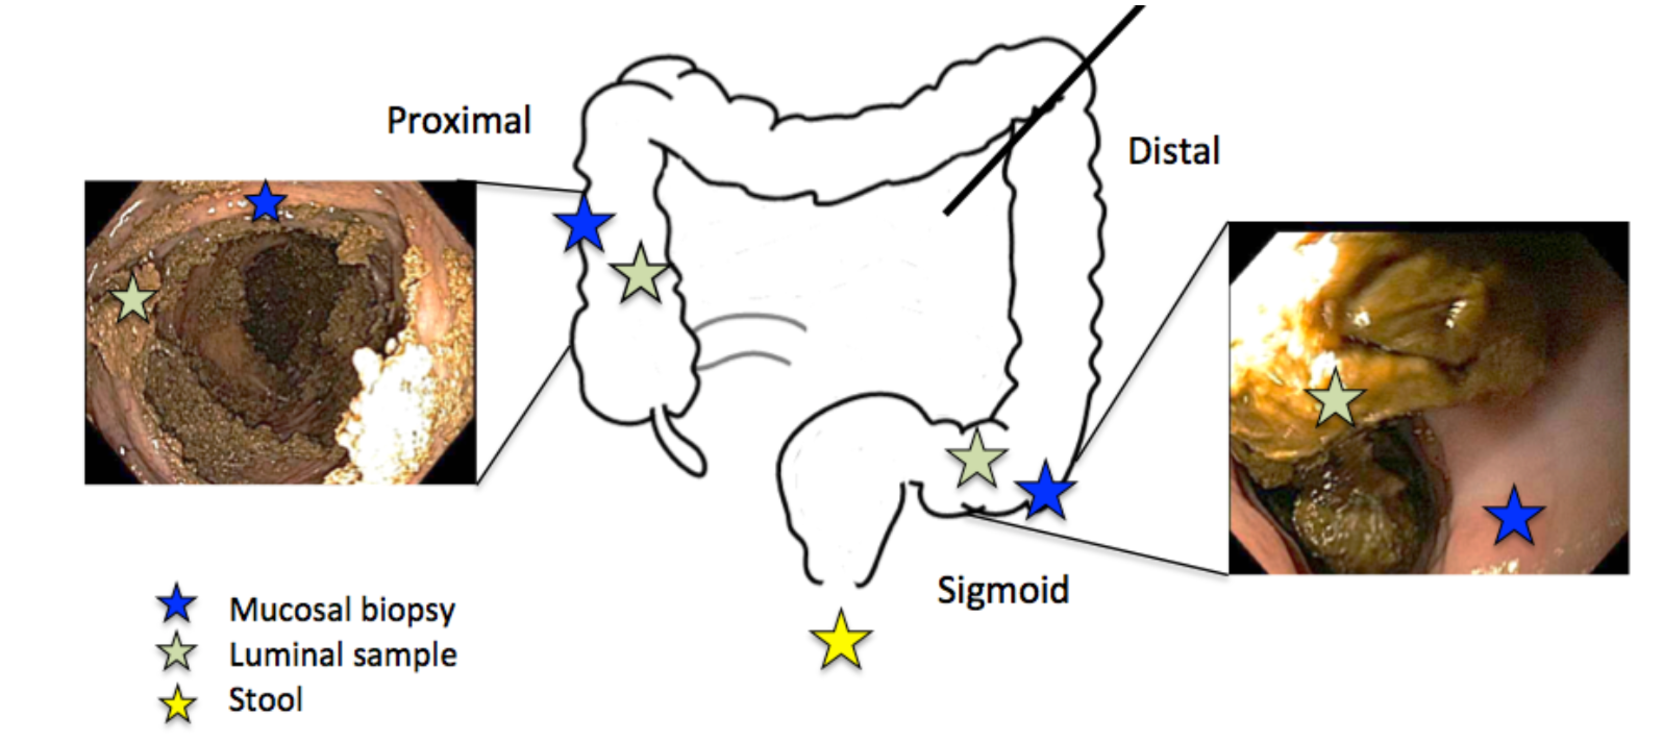
\includegraphics{../submission/figure_1.pdf}

Sampling strategy. A flexible sigmoidoscope was used to sample the
distal colonic luminal contents and mucosa. The scope was inserted
\textasciitilde{} 25cm into the subject and endoscopy brushes were used
to sample the luminal contents (green star). A separate set of biopsy
forceps was used to sample the distal mucosa (blue star). The
sigmoidoscope was removed. A pediatric colonoscope was inserted and used
to access the proximal colon. Biopsies were taken of the proximal
luminal contents and mucosa as described. One week prior to the
procedure stool was collected at home and sent into the laboratory.
Representative images from one individual are shown.

\newpage

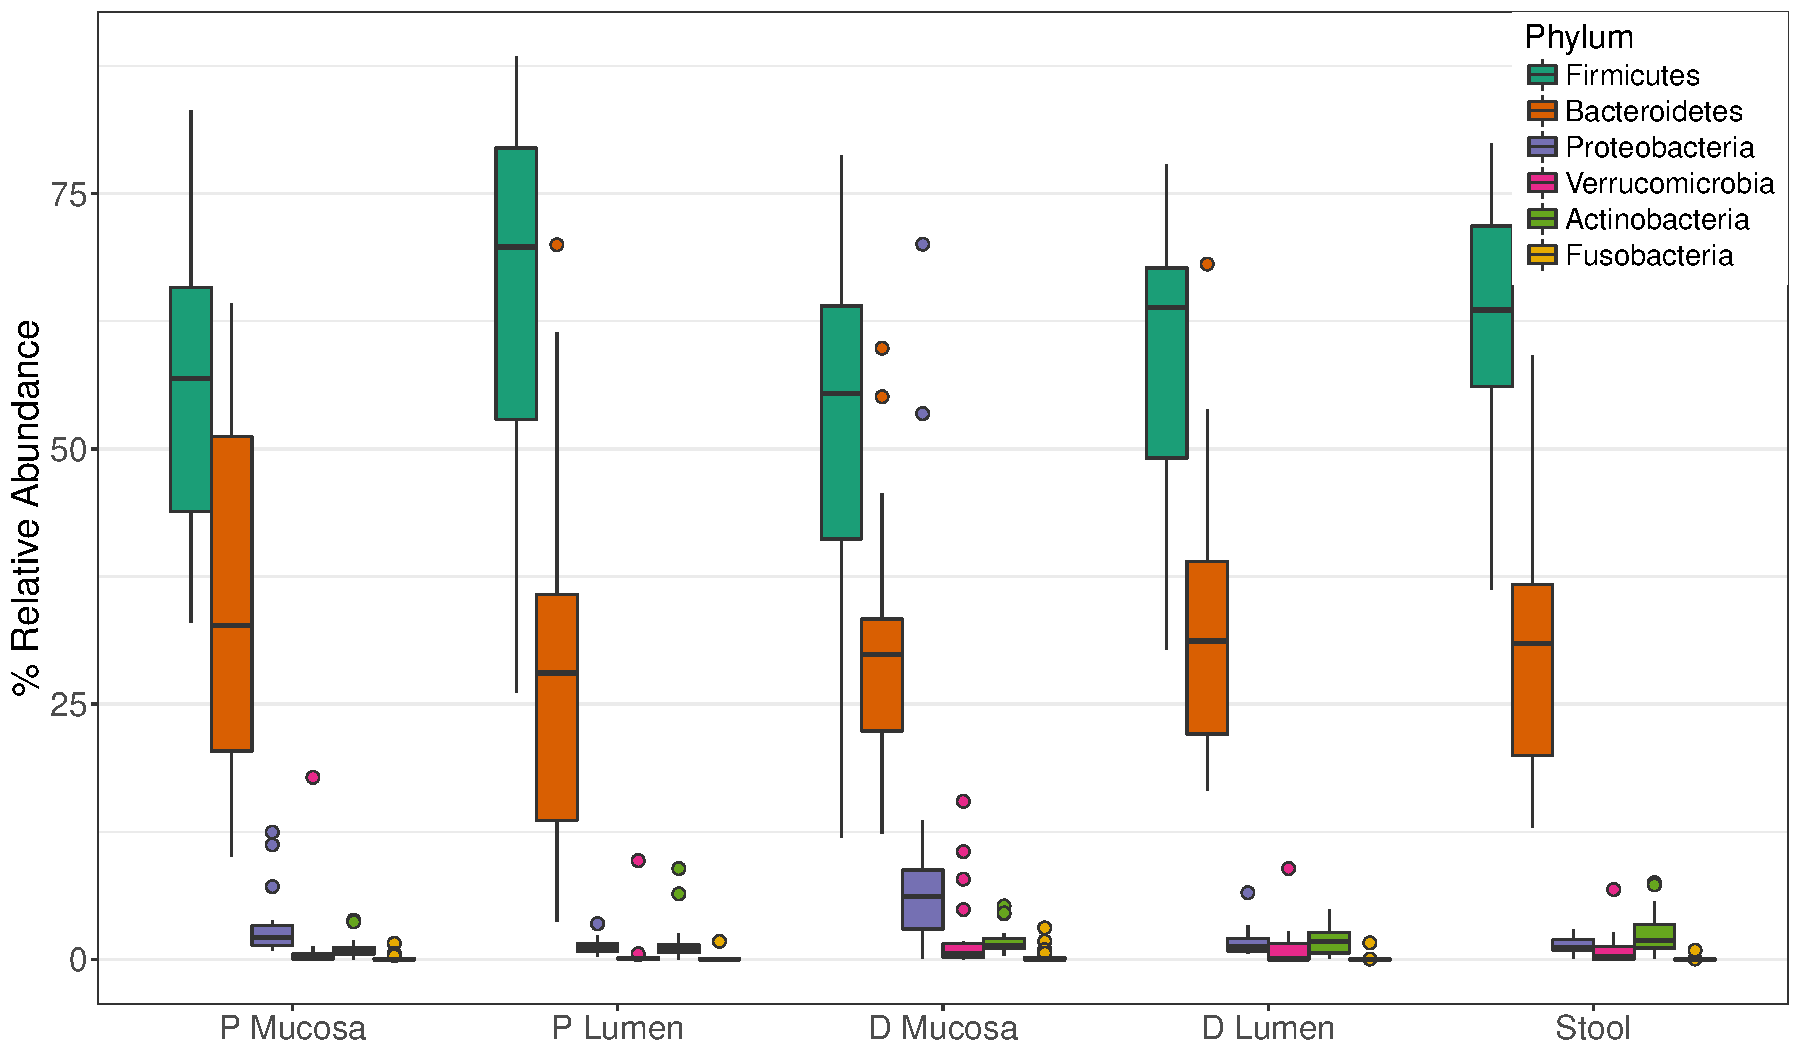
\includegraphics{../submission/figure_2.pdf}

\paragraph{Figure 2}\label{figure-2}

Microbial membership and diversity of the proximal and distal human
colon. A) Relative abundance of the top five bacterial phyla in each
sampling site. Each box represents the median and confidence intervals.
B) Simpson diversity of the microbial communities at each location. The
lines represent the median values.

\newpage

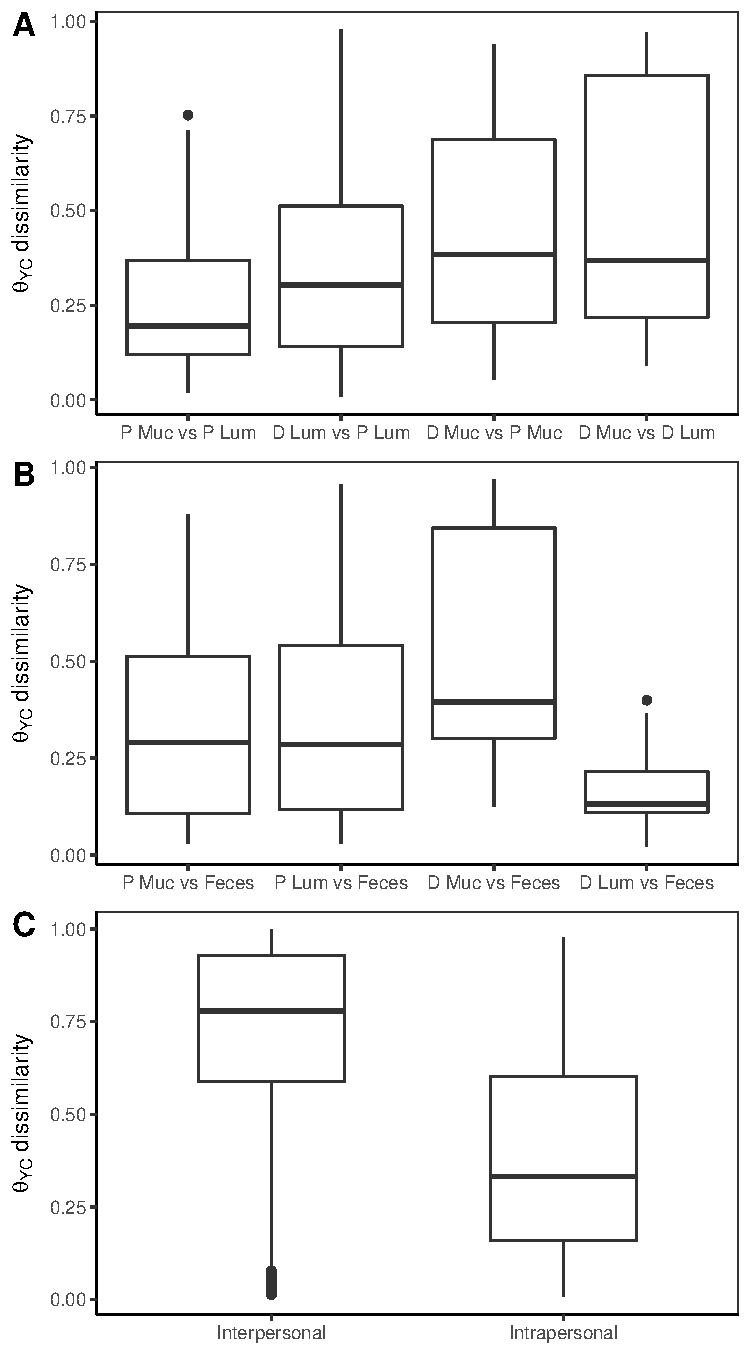
\includegraphics{../submission/figure_3.pdf}

\paragraph{Figure 3}\label{figure-3}

Distances of microbial community structure between sites of the gut.
ThetaYC distances are shown for interpersonal similarities between two
sites -- each point represents one individual. In (A), comparisons of
the proximal and distal mucosal and lumen are shown. In (B), comparisons
of each site to the exit stool are shown.

\newpage

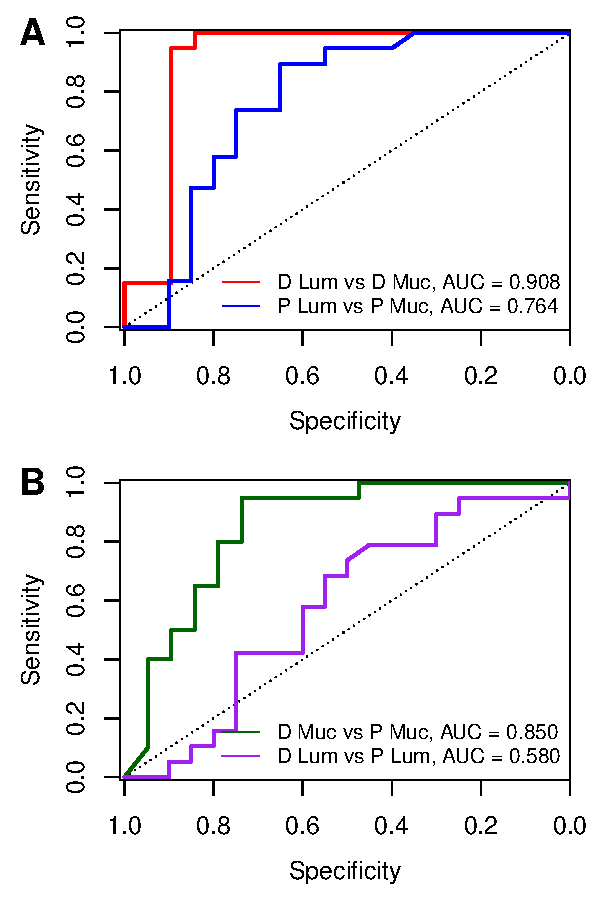
\includegraphics{../submission/figure_4.pdf}

\paragraph{Figure 4}\label{figure-4}

Taxa specific to the distal and proximal sides of the colon. Top five
OTUs that are most important for the classification model for the distal
mucosa and lumen (A) and the proximal mucosa and lumen (B).

\newpage

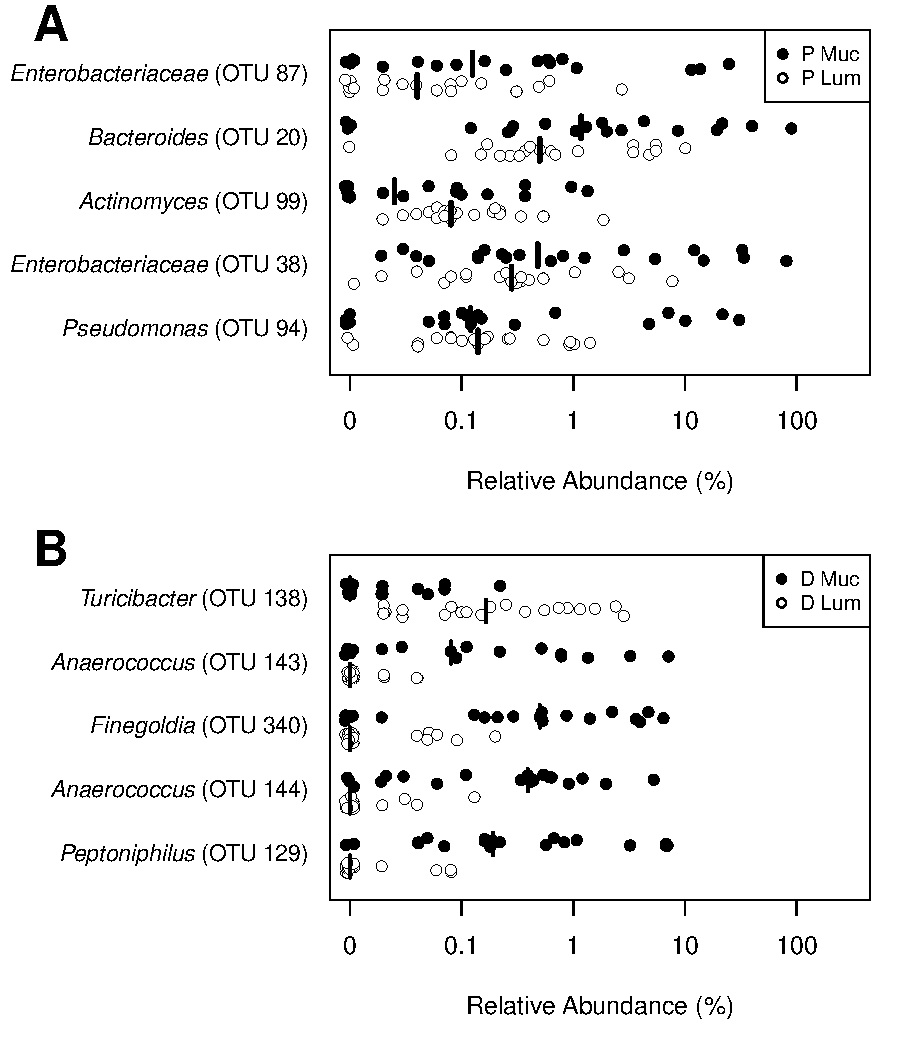
\includegraphics{../submission/figure_5.pdf}

\paragraph{Figure 5}\label{figure-5}

Taxa specific to the distal and proximal mucosa and lumen. Top five OTUs
that are most important for the classification model for the distal and
proximal mucosa (A) and the distal and proximal lumen (B).

\newpage

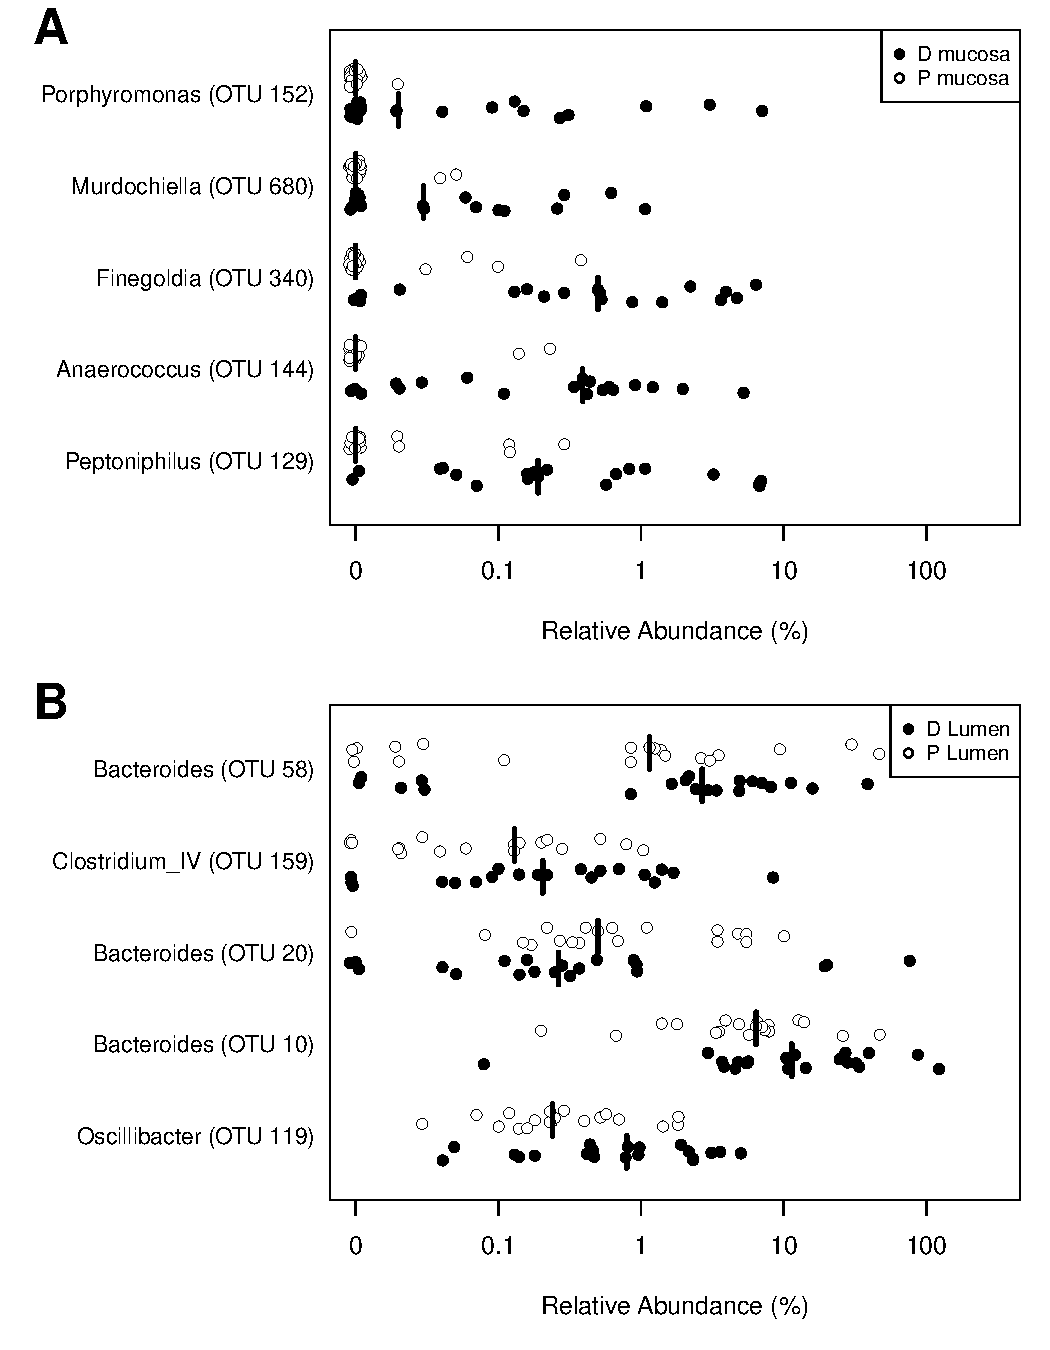
\includegraphics{../submission/figure_6.pdf}

\paragraph{Figure 6}\label{figure-6}

Location and abundance of cancer-associated OTUs. Relative abundance was
calculated and plotted by sample site for each OTU of interest: (A)
\emph{Fusobacterium nucleatum subsp. animalis} (B) \emph{Fusobacterium
varium} and (C) \emph{Porphyromonas asacharolytica}

\newpage

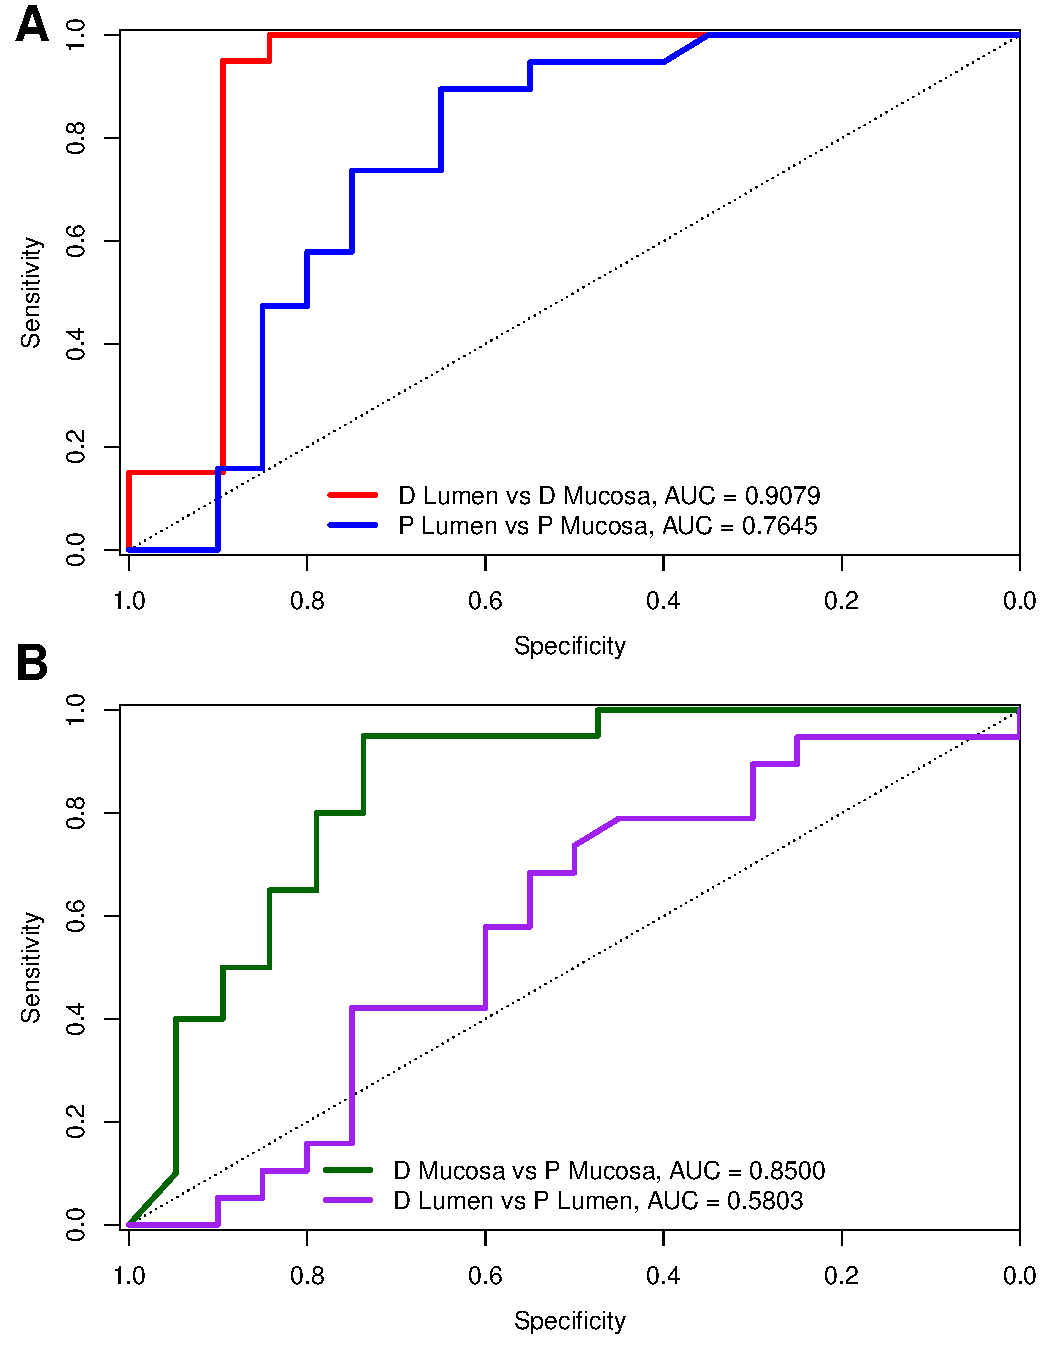
\includegraphics{../submission/figure_S1.pdf}

\paragraph{Figure S1}\label{figure-s1}

Random Forest classifies locations in the colon. A) Receiver Operator
Characteristic curves are shown for the 10-fold cross validation of the
Random Forest model classifying distal lumen versus proximal lumen
(orange) and distal mucosa vs proximal mucosa (green). (B) Receiver
Operator Characteristic curves are shown for the 10-fold cross
validation of the Random Forest model classifying lumen and mucosal
samples for the distal (red) and proximal (blue) sides of the colon.

\subsubsection*{References}\label{references}
\addcontentsline{toc}{subsubsection}{References}

\hypertarget{refs}{}
\hypertarget{ref-Yamauchi2012}{}
1. \textbf{Yamauchi M}, \textbf{Lochhead P}, \textbf{Morikawa T},
\textbf{Huttenhower C}, \textbf{Chan AT}, \textbf{Giovannucci E},
\textbf{Fuchs C}, \textbf{Ogino S}. 2012. Colorectal cancer: A tale of
two sides or a continuum?: Figure 1. Gut \textbf{61}:794--797.
doi:\href{https://doi.org/10.1136/gutjnl-2012-302014}{10.1136/gutjnl-2012-302014}.

\hypertarget{ref-Forbes2016}{}
2. \textbf{Forbes JD}, \textbf{Domselaar GV}, \textbf{Bernstein CN}.
2016. The gut microbiota in immune-mediated inflammatory diseases.
Frontiers in Microbiology \textbf{7}.
doi:\href{https://doi.org/10.3389/fmicb.2016.01081}{10.3389/fmicb.2016.01081}.

\hypertarget{ref-Halfvarson2017}{}
3. \textbf{Halfvarson J}, \textbf{Brislawn CJ}, \textbf{Lamendella R},
\textbf{Vazquez-Baeza Y}, \textbf{Walters WA}, \textbf{Bramer LM},
\textbf{DAmato M}, \textbf{Bonfiglio F}, \textbf{McDonald D},
\textbf{Gonzalez A}, \textbf{McClure EE}, \textbf{Dunklebarger MF},
\textbf{Knight R}, \textbf{Jansson JK}. 2017. Dynamics of the human gut
microbiome in inflammatory bowel disease. Nature Microbiology
\textbf{2}:17004.
doi:\href{https://doi.org/10.1038/nmicrobiol.2017.4}{10.1038/nmicrobiol.2017.4}.

\hypertarget{ref-Benedix2010}{}
4. \textbf{Benedix F}, \textbf{Kube R}, \textbf{Meyer F},
\textbf{Schmidt U}, \textbf{Gastinger I}, \textbf{Lippert H}. 2010.
Comparison of 17, 641 patients with right- and left-sided colon cancer:
Differences in epidemiology, perioperative course, histology, and
survival. Diseases of the Colon \& Rectum \textbf{53}:57--64.
doi:\href{https://doi.org/10.1007/dcr.0b013e3181c703a4}{10.1007/dcr.0b013e3181c703a4}.

\hypertarget{ref-Albenberg2014}{}
5. \textbf{Albenberg L}, \textbf{Esipova TV}, \textbf{Judge CP},
\textbf{Bittinger K}, \textbf{Chen J}, \textbf{Laughlin A},
\textbf{Grunberg S}, \textbf{Baldassano RN}, \textbf{Lewis JD},
\textbf{Li H}, \textbf{Thom SR}, \textbf{Bushman FD}, \textbf{Vinogradov
SA}, \textbf{Wu GD}. 2014. Correlation between intraluminal oxygen
gradient and radial partitioning of intestinal microbiota.
Gastroenterology \textbf{147}:1055--1063.e8.
doi:\href{https://doi.org/10.1053/j.gastro.2014.07.020}{10.1053/j.gastro.2014.07.020}.

\hypertarget{ref-Donaldson2015}{}
6. \textbf{Donaldson GP}, \textbf{Lee SM}, \textbf{Mazmanian SK}. 2015.
Gut biogeography of the bacterial microbiota. Nature Reviews
Microbiology \textbf{14}:20--32.
doi:\href{https://doi.org/10.1038/nrmicro3552}{10.1038/nrmicro3552}.

\hypertarget{ref-Dejea2014}{}
7. \textbf{Dejea CM}, \textbf{Wick EC}, \textbf{Hechenbleikner EM},
\textbf{White JR}, \textbf{Welch JLM}, \textbf{Rossetti BJ},
\textbf{Peterson SN}, \textbf{Snesrud EC}, \textbf{Borisy GG},
\textbf{Lazarev M}, \textbf{Stein E}, \textbf{Vadivelu J},
\textbf{Roslani AC}, \textbf{Malik AA}, \textbf{Wanyiri JW}, \textbf{Goh
KL}, \textbf{Thevambiga I}, \textbf{Fu K}, \textbf{Wan F}, \textbf{Llosa
N}, \textbf{Housseau F}, \textbf{Romans K}, \textbf{Wu X},
\textbf{McAllister FM}, \textbf{Wu S}, \textbf{Vogelstein B},
\textbf{Kinzler KW}, \textbf{Pardoll DM}, \textbf{Sears CL}. 2014.
Microbiota organization is a distinct feature of proximal colorectal
cancers. Proceedings of the National Academy of Sciences
\textbf{111}:18321--18326.
doi:\href{https://doi.org/10.1073/pnas.1406199111}{10.1073/pnas.1406199111}.

\hypertarget{ref-Baxter2016}{}
8. \textbf{Baxter NT}, \textbf{Ruffin MT}, \textbf{Rogers MAM},
\textbf{Schloss PD}. 2016. Microbiota-based model improves the
sensitivity of fecal immunochemical test for detecting colonic lesions.
Genome Medicine \textbf{8}.
doi:\href{https://doi.org/10.1186/s13073-016-0290-3}{10.1186/s13073-016-0290-3}.

\hypertarget{ref-Strauss2011}{}
9. \textbf{Strauss J}, \textbf{Kaplan GG}, \textbf{Beck PL},
\textbf{Rioux K}, \textbf{Panaccione R}, \textbf{DeVinney R},
\textbf{Lynch T}, \textbf{Allen-Vercoe E}. 2011. Invasive potential of
gut mucosa-derived fusobacterium nucleatum positively correlates with
IBD status of the host. Inflammatory Bowel Diseases
\textbf{17}:1971--1978.
doi:\href{https://doi.org/10.1002/ibd.21606}{10.1002/ibd.21606}.

\hypertarget{ref-Jalanka2014}{}
10. \textbf{Jalanka J}, \textbf{Salonen A}, \textbf{Salojärvi J},
\textbf{Ritari J}, \textbf{Immonen O}, \textbf{Marciani L},
\textbf{Gowland P}, \textbf{Hoad C}, \textbf{Garsed K}, \textbf{Lam C},
\textbf{Palva A}, \textbf{Spiller RC}, \textbf{Vos WM de}. 2014. Effects
of bowel cleansing on the intestinal microbiota. Gut
\textbf{64}:1562--1568.
doi:\href{https://doi.org/10.1136/gutjnl-2014-307240}{10.1136/gutjnl-2014-307240}.

\hypertarget{ref-Harrell2012}{}
11. \textbf{Harrell L}, \textbf{Wang Y}, \textbf{Antonopoulos D},
\textbf{Young V}, \textbf{Lichtenstein L}, \textbf{Huang Y},
\textbf{Hanauer S}, \textbf{Chang E}. 2012. Standard colonic lavage
alters the natural state of mucosal-associated microbiota in the human
colon. PLoS ONE \textbf{7}:e32545.
doi:\href{https://doi.org/10.1371/journal.pone.0032545}{10.1371/journal.pone.0032545}.

\hypertarget{ref-LloydPrice2016}{}
12. \textbf{Lloyd-Price J}, \textbf{Abu-Ali G}, \textbf{Huttenhower C}.
2016. The healthy human microbiome. Genome Medicine \textbf{8}.
doi:\href{https://doi.org/10.1186/s13073-016-0307-y}{10.1186/s13073-016-0307-y}.

\hypertarget{ref-Eckburg2005}{}
13. \textbf{Eckburg PB}. 2005. Diversity of the human intestinal
microbial flora. Science \textbf{308}:1635--1638.
doi:\href{https://doi.org/10.1126/science.1110591}{10.1126/science.1110591}.

\hypertarget{ref-deCarcer2010}{}
14. \textbf{Cárcer DA de}, \textbf{Cuív PÓ}, \textbf{Wang T},
\textbf{Kang S}, \textbf{Worthley D}, \textbf{Whitehall V},
\textbf{Gordon I}, \textbf{McSweeney C}, \textbf{Leggett B},
\textbf{Morrison M}. 2010. Numerical ecology validates a biogeographical
distribution and gender-based effect on mucosa-associated bacteria along
the human colon. The ISME Journal \textbf{5}:801--809.
doi:\href{https://doi.org/10.1038/ismej.2010.177}{10.1038/ismej.2010.177}.

\hypertarget{ref-Zhang2013}{}
15. \textbf{Zhang Z}, \textbf{Geng J}, \textbf{Tang X}, \textbf{Fan H},
\textbf{Xu J}, \textbf{Wen X}, \textbf{Ma Z (Sam)}, \textbf{Shi P}.
2013. Spatial heterogeneity and co-occurrence patterns of human
mucosal-associated intestinal microbiota. The ISME Journal
\textbf{8}:881--893.
doi:\href{https://doi.org/10.1038/ismej.2013.185}{10.1038/ismej.2013.185}.

\hypertarget{ref-Castellarin2011}{}
16. \textbf{Castellarin M}, \textbf{Warren RL}, \textbf{Freeman JD},
\textbf{Dreolini L}, \textbf{Krzywinski M}, \textbf{Strauss J},
\textbf{Barnes R}, \textbf{Watson P}, \textbf{Allen-Vercoe E},
\textbf{Moore RA}, \textbf{Holt RA}. 2011. Fusobacterium nucleatum
infection is prevalent in human colorectal carcinoma. Genome Research
\textbf{22}:299--306.
doi:\href{https://doi.org/10.1101/gr.126516.111}{10.1101/gr.126516.111}.

\hypertarget{ref-Lee2016}{}
17. \textbf{Lee Y}, \textbf{Eun CS}, \textbf{Lee AR}, \textbf{Park CH},
\textbf{Han DS}. 2016. FusobacteriumIsolates recovered from colonic
biopsies of inflammatory bowel disease patients in korea. Annals of
Laboratory Medicine \textbf{36}:387.
doi:\href{https://doi.org/10.3343/alm.2016.36.4.387}{10.3343/alm.2016.36.4.387}.

\hypertarget{ref-Hong2011}{}
18. \textbf{Hong P-Y}, \textbf{Croix JA}, \textbf{Greenberg E},
\textbf{Gaskins HR}, \textbf{Mackie RI}. 2011. Pyrosequencing-based
analysis of the mucosal microbiota in healthy individuals reveals
ubiquitous bacterial groups and micro-heterogeneity. PLoS ONE
\textbf{6}:e25042.
doi:\href{https://doi.org/10.1371/journal.pone.0025042}{10.1371/journal.pone.0025042}.

\hypertarget{ref-Stearns2011}{}
19. \textbf{Stearns JC}, \textbf{Lynch MDJ}, \textbf{Senadheera DB},
\textbf{Tenenbaum HC}, \textbf{Goldberg MB}, \textbf{Cvitkovitch DG},
\textbf{Croitoru K}, \textbf{Moreno-Hagelsieb G}, \textbf{Neufeld JD}.
2011. Bacterial biogeography of the human digestive tract. Scientific
Reports \textbf{1}.
doi:\href{https://doi.org/10.1038/srep00170}{10.1038/srep00170}.

\hypertarget{ref-Sears2014}{}
20. \textbf{Sears CL}, \textbf{Garrett WS}. 2014. Microbes, microbiota,
and colon cancer. Cell Host \& Microbe \textbf{15}:317--328.
doi:\href{https://doi.org/10.1016/j.chom.2014.02.007}{10.1016/j.chom.2014.02.007}.

\hypertarget{ref-Mima2016}{}
21. \textbf{Mima K}, \textbf{Cao Y}, \textbf{Chan AT}, \textbf{Qian ZR},
\textbf{Nowak JA}, \textbf{Masugi Y}, \textbf{Shi Y}, \textbf{Song M},
\textbf{Silva A da}, \textbf{Gu M}, \textbf{Li W}, \textbf{Hamada T},
\textbf{Kosumi K}, \textbf{Hanyuda A}, \textbf{Liu L}, \textbf{Kostic
AD}, \textbf{Giannakis M}, \textbf{Bullman S}, \textbf{Brennan CA},
\textbf{Milner DA}, \textbf{Baba H}, \textbf{Garraway LA},
\textbf{Meyerhardt JA}, \textbf{Garrett WS}, \textbf{Huttenhower C},
\textbf{Meyerson M}, \textbf{Giovannucci EL}, \textbf{Fuchs CS},
\textbf{Nishihara R}, \textbf{Ogino S}. 2016. Fusobacterium nucleatum in
colorectal carcinoma tissue according to tumor location. Clinical and
Translational Gastroenterology \textbf{7}:e200.
doi:\href{https://doi.org/10.1038/ctg.2016.53}{10.1038/ctg.2016.53}.

\hypertarget{ref-Whitmore2014}{}
22. \textbf{Whitmore SE}, \textbf{Lamont RJ}. 2014. Oral bacteria and
cancer. PLoS Pathogens \textbf{10}:e1003933.
doi:\href{https://doi.org/10.1371/journal.ppat.1003933}{10.1371/journal.ppat.1003933}.

\hypertarget{ref-Flynn2016}{}
23. \textbf{Flynn KJ}, \textbf{Baxter NT}, \textbf{Schloss PD}. 2016.
Metabolic and community synergy of oral bacteria in colorectal cancer.
mSphere \textbf{1}:e00102--16.
doi:\href{https://doi.org/10.1128/msphere.00102-16}{10.1128/msphere.00102-16}.

\hypertarget{ref-Dharmani2011}{}
24. \textbf{Dharmani P}, \textbf{Strauss J}, \textbf{Ambrose C},
\textbf{Allen-Vercoe E}, \textbf{Chadee K}. 2011. Fusobacterium
nucleatum infection of colonic cells stimulates MUC2 mucin and tumor
necrosis factor alpha. Infection and Immunity \textbf{79}:2597--2607.
doi:\href{https://doi.org/10.1128/iai.05118-11}{10.1128/iai.05118-11}.

\hypertarget{ref-Ohkusa2003}{}
25. \textbf{Ohkusa T}. 2003. Induction of experimental ulcerative
colitis by fusobacterium varium isolated from colonic mucosa of patients
with ulcerative colitis. Gut \textbf{52}:79--83.
doi:\href{https://doi.org/10.1136/gut.52.1.79}{10.1136/gut.52.1.79}.

\hypertarget{ref-Ohkusa2002}{}
26. \textbf{Ohkusa T}, \textbf{Sato N}, \textbf{Ogihara T},
\textbf{Morita K}, \textbf{Ogawa M}, \textbf{Okayasu I}. 2002.
Fusobacterium varium localized in the colonic mucosa of patients with
ulcerative colitis stimulates species-specific antibody. Journal of
Gastroenterology and Hepatology \textbf{17}:849--853.
doi:\href{https://doi.org/10.1046/j.1440-1746.2002.02834.x}{10.1046/j.1440-1746.2002.02834.x}.

\hypertarget{ref-Shobar2016}{}
27. \textbf{Shobar RM}, \textbf{Velineni S}, \textbf{Keshavarzian A},
\textbf{Swanson G}, \textbf{DeMeo MT}, \textbf{Melson JE},
\textbf{Losurdo J}, \textbf{Engen PA}, \textbf{Sun Y}, \textbf{Koenig
L}, \textbf{Mutlu EA}. 2016. The effects of bowel preparation on
microbiota-related metrics differ in health and in inflammatory bowel
disease and for the mucosal and luminal microbiota compartments.
Clinical and Translational Gastroenterology \textbf{7}:e143.
doi:\href{https://doi.org/10.1038/ctg.2015.54}{10.1038/ctg.2015.54}.

\hypertarget{ref-Kozich2013}{}
28. \textbf{Kozich JJ}, \textbf{Westcott SL}, \textbf{Baxter NT},
\textbf{Highlander SK}, \textbf{Schloss PD}. 2013. Development of a
dual-index sequencing strategy and curation pipeline for analyzing
amplicon sequence data on the MiSeq illumina sequencing platform.
Applied and Environmental Microbiology \textbf{79}:5112--5120.
doi:\href{https://doi.org/10.1128/aem.01043-13}{10.1128/aem.01043-13}.

\hypertarget{ref-Schloss2009}{}
29. \textbf{Schloss PD}, \textbf{Westcott SL}, \textbf{Ryabin T},
\textbf{Hall JR}, \textbf{Hartmann M}, \textbf{Hollister EB},
\textbf{Lesniewski RA}, \textbf{Oakley BB}, \textbf{Parks DH},
\textbf{Robinson CJ}, \textbf{Sahl JW}, \textbf{Stres B},
\textbf{Thallinger GG}, \textbf{Horn DJV}, \textbf{Weber CF}. 2009.
Introducing mothur: Open-source, platform-independent,
community-supported software for describing and comparing microbial
communities. Applied and Environmental Microbiology
\textbf{75}:7537--7541.
doi:\href{https://doi.org/10.1128/aem.01541-09}{10.1128/aem.01541-09}.

\hypertarget{ref-Wang2007}{}
30. \textbf{Wang Q}, \textbf{Garrity GM}, \textbf{Tiedje JM},
\textbf{Cole JR}. 2007. Naive bayesian classifier for rapid assignment
of rRNA sequences into the new bacterial taxonomy. Applied and
Environmental Microbiology \textbf{73}:5261--5267.
doi:\href{https://doi.org/10.1128/aem.00062-07}{10.1128/aem.00062-07}.

\hypertarget{ref-Liaw2002}{}
31. \textbf{Liaw A}, \textbf{Wiener M}. 2002. Classification and
regression by randomForest. R News: The Newsletter of the R Project
\textbf{2}:18--22.


\end{document}
